\section{Implementation Approach}

The project was implemented following an incremental development strategy with the following components:
\begin{enumerate}
    \item \textbf{Simulation Engine}: Basic CARLA connection, vehicle spawning, and synchronous simulation loop
    \item \textbf{Object Detection}: Integration of YOLOv8 for pedestrian detection
    \item \textbf{Depth Processing}: Conversion of depth camera data to normalized distance map
    \item \textbf{Kalman Tracking}: Implementation of 2D trajectory Kalman filter for object tracking
    \item \textbf{Collision Assessment}: TTC-based collision risk calculation
    \item \textbf{Control Logic}: Velocity-based braking decision
    \item \textbf{Visualization}: Real-time display of detections and predictions
    \item \textbf{Scenarios}: Definition and validation of test scenarios
\end{enumerate}

\section{Unit Tests}

The project includes a comprehensive test suite of 98 unit tests covering collision assessment, Kalman filtering, scenario validation, perception, configuration loading, state management, and sensor lifecycle. A detailed breakdown of test files and coverage is provided in the Deployment chapter.

\section{Functional Analysis}

\subsection{Detection Pipeline}

The perception pipeline consists of three main stages:

\begin{figure}[h]
    \centering
    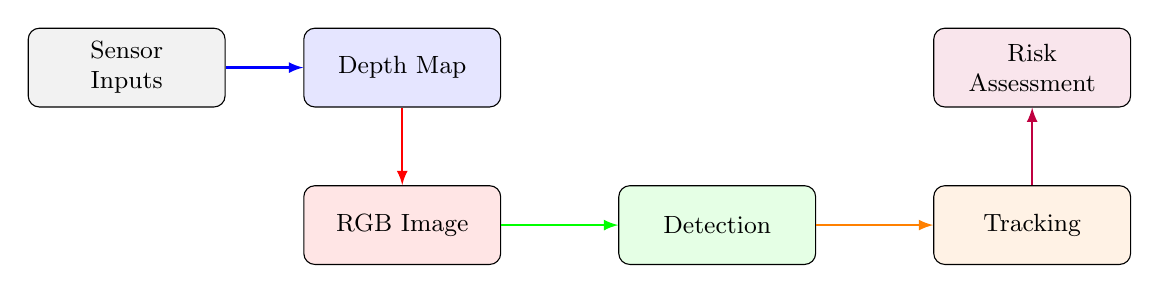
\begin{tikzpicture}[>=latex]
        \tikzset{
            block/.style={draw, rounded corners, minimum height=1cm, minimum width=2.5cm, align=center, font=\small},
            arrow/.style={->, thick}
        }
        
        \node[block, fill=gray!10] (input) at (0, 0) {Sensor\\Inputs};
        \node[block, fill=blue!10] (depth) at (3.5, 0) {Depth Map};
        \node[block, fill=red!10] (img) at (3.5, -2) {RGB Image};
        \node[block, fill=green!10] (detect) at (7.5, -2) {Detection};
        \node[block, fill=orange!10] (kalman) at (11.5, -2) {Tracking};
        \node[block, fill=purple!10] (risk) at (11.5, 0) {Risk\\Assessment};
        
        \draw[arrow, blue] (input) -- (depth);
        \draw[arrow, red] (depth) -- (img);
        \draw[arrow, green] (img) -- (detect);
        \draw[arrow, orange] (detect) -- (kalman);
        \draw[arrow, purple] (kalman) -- (risk);
    \end{tikzpicture}
    \caption{Perception pipeline data flow}
\end{figure}

\textbf{Stage 1: Depth Processing}\\
Depth images are normalized to meters using:
\begin{verbatim}
normalized_depth = (R + G * 256 + B * 256 * 256) / 256^3
depth_meters = normalized_depth * 1000
\end{verbatim}

\textbf{Stage 2: Object Detection}\\
YOLOv8 tracks objects across frames and returns:
\begin{itemize}
    \item Bounding boxes (x1, y1, x2, y2) in image coordinates
    \item Confidence scores for each detection
    \item Class IDs (0: person)
    \item Track IDs for persistent tracking across frames
\end{itemize}

\textbf{Stage 3: Kalman Tracking}\\
For each detected object:
\begin{enumerate}
    \item Calculate object's 3D position (X, Z) using depth map
    \item Initialize or update Kalman filter with current position
    \item Predict object trajectory to future frames
    \item Compute velocity relative to ego vehicle
\end{enumerate}

\subsection{Kalman Filter Performance}

The 4-state Kalman filter executes predict-correct cycles at the simulation frequency (50ms intervals). The mathematical formulation, matrices, and state vectors are detailed in the Tracking Algorithm section.

In terms of performance, the filter successfully:
\begin{itemize}
    \item Filters high-frequency noise from raw camera depth observations.
    \item Smooths the estimated trajectory of the pedestrian.
    \item Estimates the lateral and longitudinal velocities ($V_{x}, V_{z}$) implicitly from the position history.
\end{itemize}

By compensating for ego-motion using the control inputs, the velocity estimations represent the relative velocities of the pedestrian accurately. This allows for stable relative velocity calculations which are critical for the subsequent Time-to-Collision (TTC) estimation.

\subsection{Model Quality Evaluation}

To evaluate the performance of the perception and tracking pipeline, we extracted the true 3D spatial parameters from the CARLA simulator's odometry and compared them against the estimates produced by the Kalman filter. Figure~\ref{fig:eval_results} illustrates the system's performance over a 150-frame sequence in the \texttt{colliding-pedestrian} scenario.
\clearpage
\begin{figure}[h]
    \centering
    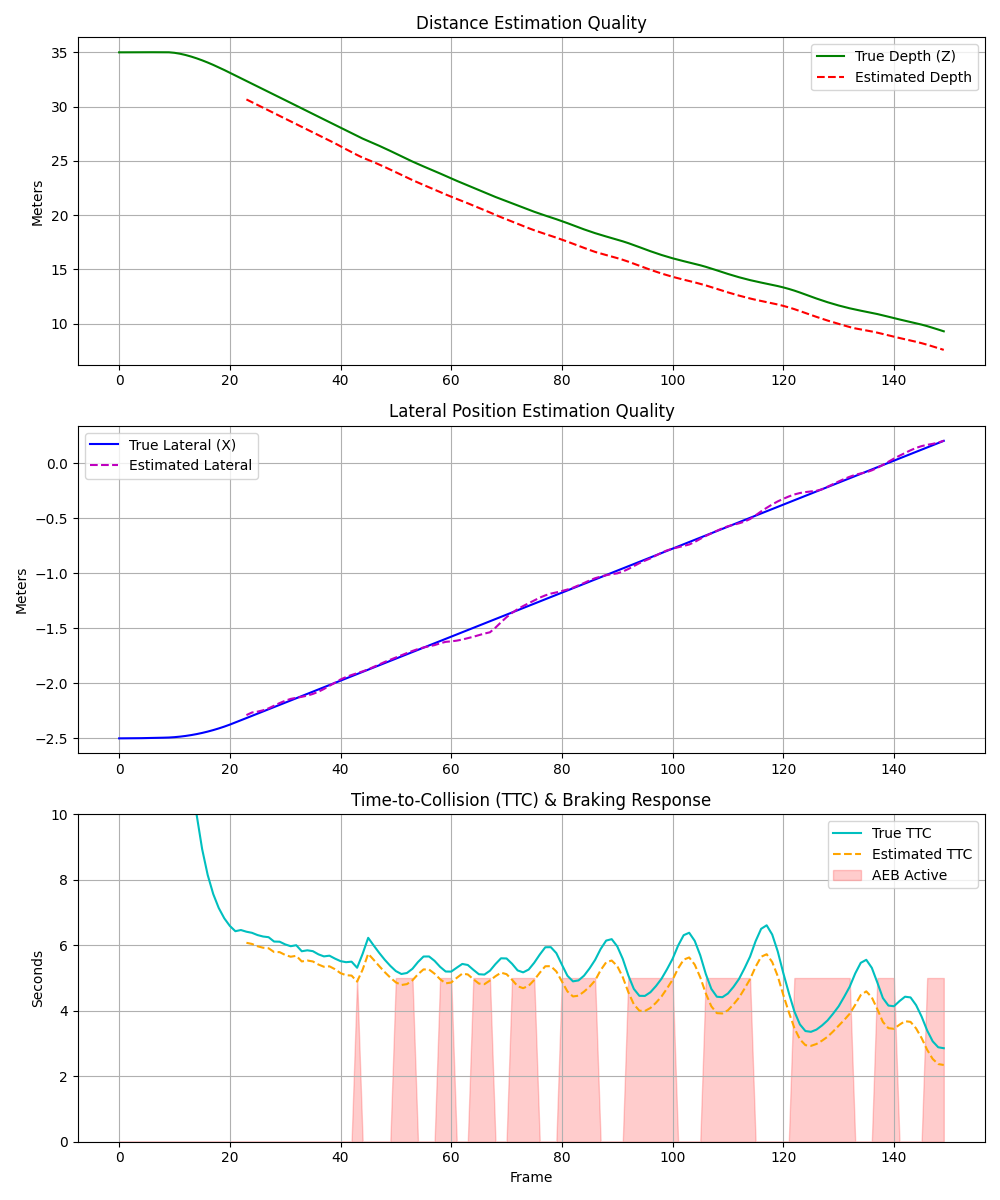
\includegraphics[width=0.9\textwidth]{assets/evaluation_results.png}
    \caption{Model evaluation: True vs. Estimated tracking performance and TTC.}
    \label{fig:eval_results}
\end{figure}

The depth estimation closely tracks the ground truth, effectively filtering out sensor noise. The lateral position estimation demonstrates accurate tracking of the pedestrian's movement into the ego-vehicle's path. Furthermore, the Time-to-Collision (TTC) metric rapidly converges as the pedestrian enters the vehicle's trajectory, successfully triggering the Automatic Emergency Braking (AEB) well in advance of the potential impact.

\subsection{Collision Risk Assessment}

The collision assessment module uses a geometric approach based on predicted trajectories:

\begin{enumerate}
    \item \textbf{Time-to-Collision (TTC)}:
    \begin{equation}
        TTC = \frac{Z}{|v_{relative}|}
    \end{equation}
    where $Z$ is the depth distance and $v_{relative}$ is the closing speed.
    
    \item \textbf{Lateral Position at Impact}:
    \begin{equation}
        X_{impact} = X + v_{relative\_lateral} \cdot TTC
    \end{equation}
    
    \item \textbf{Hitbox Check}:
    $ |X_{impact}| \leq car\textunderscore half\textunderscore width + margin$ 
\end{enumerate}

The system triggers braking when:
\begin{itemize}
    \item TTC $<$ 5.0 seconds (collision within 5 seconds)
    \item Lateral position at impact is within car hitbox plus safety margin
\end{itemize}

\section{Scenario Validation}

We defined two scenarios for testing:

\begin{table}[h]
    \centering
    \begin{tabular}{|l|l|l|l|l|}
        \hline
        Parameter & non-colliding & colliding & Type & Default \\
        \hline
        walker\_distance\_from\_vehicle & 35.0m & 35.0m & float & 35.0 \\
        \hline
        walker\_height & 1.0m & 1.0m & float & 1.0 \\
        \hline
        walker\_horizontal\_offset & +5.0m & -2.5m & float & 0.0 \\
        \hline
        walker\_speed & 2.0 m/s & 0.4 m/s & float & 1.0 \\
        \hline
        target\_speed\_mps & 5.56 m/s & 5.56 m/s & float & 5.56 \\
        \hline
        prediction\_future\_frames & 30 & 30 & int & 30 \\
        \hline
    \end{tabular}
    \caption{Scenario parameters for non-colliding and colliding pedestrian cases}
\end{table}

The validation ensures:
\begin{itemize}
    \item All required fields are present
    \item All numeric values are of correct type
    \item Speeds are positive and non-zero
    \item Horizontal offset can be positive (right), negative (left), or zero (directly in front)
\end{itemize}


\section{Examples}
These are some examples of the project's results:
\clearpage
\begin{figure}[h!]
    
\includegraphics[width=\textwidth]{two_pedestrian_complete.png}
    \centering
    \label{fig:two_pedestrian_crossing_complete}
    \caption{Complete application, with Carla, PyGame window and Terminal output}
\end{figure}

In \ref{fig:two_pedestrian_crossing_complete} we can see the whole system running, actively braking to avoid collision with the pedestrian crossing, as seen by the vehicle's brake lights.
\clearpage
\begin{figure}[!h]
    
\includegraphics[width=\textwidth]{two_pedestrian_pygame.png}
    \centering
    \label{fig:two_pedestrian_crossing_pygame}
    \caption{PyGame window}
\end{figure}

In \ref{fig:two_pedestrian_crossing_pygame}'s view, representing the vehicle's front RGB camera, with kalman's prediction we have enhanced the feed to show the future positions of the pedestrian.
\section{Known Limitations}

\begin{enumerate}
    \item \textbf{Pedestrian Model}: The simulation uses a simple \texttt{walker} actor that moves independently. Realistic pedestrian behavior (uncertainty, looking behavior, avoidance) would require a more sophisticated model.
    
    \item \textbf{Ego Vehicle}: The ego vehicle follows a simple speed controller without realistic autonomous driving capabilities (lane keeping, obstacle avoidance).
    
    \item \textbf{Sensor Model}: The depth camera is assumed to provide perfectly accurate depth measurements. In reality, depth sensors have noise and accuracy varies with distance.
    
    \item \textbf{YAML Limitations}: Complex scenario validation is done at runtime rather than compile-time.
    
    \item \textbf{Track Management}: Missing proper track spawning and deletion logic for handling occlusions and tracking failures.
\end{enumerate}